\documentclass[10pt,twocolumn,letterpaper]{article}
\usepackage{statcourse}
\usepackage{times}
\usepackage{epsfig}
\usepackage{graphicx}
\usepackage{amsmath}
\usepackage{amssymb}

% Include other packages here, before hyperref.

% If you comment hyperref and then uncomment it, you should delete
% egpaper.aux before re-running latex.  (Or just hit 'q' on the first latex
% run, let it finish, and you should be clear).
\usepackage[breaklinks=true,bookmarks=false,hidelinks]{hyperref}


\statcoursefinalcopy


\setcounter{page}{1}
\begin{document}

%%%%%%%%% TITLE
\title{Master's Thesis Research Proposal}

\author{Yuan Ting Lee 
\\{\tt\small Hertie School}
\\{\tt\small y.lee@mpp.hertie-school.org}
}

\maketitle

%%%%%%%%% BODY TEXT

\section{Research Paper summary}
\paragraph{Paper:} The paper selected is titled Who Leads? Who Follows? Measuring Issue Attention and Agenda
Setting by Legislators and the Mass Public Using Social Media Data by P. Barberá, A. Casas, J. Nagler, P. J. Egan, R. Bonneau, J. T. Jost, and J. A. Tucker. It was published in the American Political Science Review in 2019, and can be accessed \hyperref[https://doi.org/10.1017/S0003055419000352]{here}. \cite{barberá_2019}

\paragraph{} In this paper, the authors set out to determine whether the public or politicians lead the other in setting the political agenda. It is noteworthy in that it utilises vector autoregression (VAR) models to explore  (public's or politicians') priorities more strongly predict the relationship between citizens and politicians. The paper finds that legislators are more likely to follow, than to lead, discussion of public issues. The authors use a dataset comprising Twitter messages by legislators and the public during the 113th US Congress.

%\item If this paper proposes a solution for a particular task, clearly state what the task is.
%\item If this paper uses a particular evaluation metric (or metrics), clearly state which they are. Also state any important scores that the work achieves on these metrics (you don't have to list every single score, but if there are some key numbers, mention them).
%\item If this paper has any important models or techniques, describe them.

\paragraph{} The first task that the authors set out to do is to characterise the different issues that politicians, ordinary citizens, and media outlets discuss on Twitter, and how their importance varies over time and across groups defined by their partisanship and political interest. To do so, they use topic modelling, estimating a probabilistic model of word occurrences in documents, to infer topics from documents using a “bag-of-words” approach.

\paragraph{} Following this, the authors take advantage of the time series nature of their dataset to establish who puts issues on the agenda first by estimating a VAR model with topic-fixed effects. 

\paragraph{} The key findings of the paper are that the public was not only able to lead the expressed agenda of members of Congress, but that the magnitude of this phenomenon was greater than that associated with politicians’ ability to lead public agendas. 

\paragraph{Link to project:} Although not all the techniques used in this paper are relevant to the project, which will be discussed in the next section, key concepts such as the analysis of issues that the public pay attention to on Twitter, as well as the relationship between policy makers and the public, remain critical to the project here.

\section{Project Description}

\subsection{Motivation}

% Describe why your project is interesting. E.g., you can describe why your project could have a broader societal impact. Or, you may describe the motivation from a personal learning perspective.

% Describe the main goal(s) of your project. If possible, try to phrase this in terms of a scientific question you are trying to answer - e.g., your goal may be to investigate whether a particular model or technique performs well at a certain task, or whether you can improve a particular model by adding some new variant, or (for theoretical/analytical projects), you might have some particular hypothesis that you seek to confirm or disprove. Otherwise, your goal may be simply to successfully implement a complex model, and show that it performs well on a given task. Briefly motivate why you chose this goal - why do you think it is important, interesting, challenging and/or likely to succeed? If you have any secondary or stretch goals (i.e. things you will do if you have time), please also describe them. In this section, you should also make it clear how your project relates to your chosen paper.

This project\footnote{Github: \hyperref[https://github.com/yuantinglee/twitter-discourse]{https://github.com/yuantinglee/twitter-discourse}} will look at the public debate surrounding the process of the coal commission in Germany, and whether the multi-stakeholder process had any impact on the public debate. Several key issues that motivate the project include the following:

\subsubsection{The Coal Commission and involvement of external expertise in German policy-making}
\paragraph{} Expert commissions have been an important instrument for incorporating external expertise into political decision-making in Germany. It can be seen as an element of ``negotiation democracy", whereby the experts in the commission decide on an outcome via deliberations and negotiations. Depending on the policy field, representatives of business, science, the social partners, churches, associations and societies can be appointed and thus accelerate the later public discussion. \cite{Siefken2016}

\paragraph{} The Coal Commission, formally known as the Commission on Growth, Structural Change and Employment, is such an example of expert commissions. It was set up by the German government under the Federal Ministry for Economy and Energy (BMWi), and was tasked with developing an overarching approach to managing the coal phase-out’s technical, legal, economic and social impacts. 

\subsubsection{Polarisation on social media}
\paragraph{} At the same time, there is concern over the relationship between social media usage and political polarisation. The complex relationship between social media usage, political polarisation, and the quality of public policy/democracy is currently being studied. Questions such as how common informal political discussions occur on social media, how often such discussions occur across partisan boundaries, and the nature of the relationships of people that engage in such political discussions are key to understanding whether online platforms actually contribute to political polarisation or serve to dampen its most corrosive effects. \cite{Tucker2019}

\subsubsection{Relationship between expert commissions and public opinion}
\paragraph{} The process of the German coal commission thus presents a unique situation for analysis: is there a relationship between the ``negotiation democracy" process of such an expert commission and public opinion, as represented on social media, on the topic? Here, tweets from Twitter are used to represent public opinion on social media, in part due to their high granularity which allows for observations on swiftly changing temporal patterns on topic salience. 

\subsection{Task}

\paragraph{} The task in this project is therefore to design a method to test whether events throughout the course of the coal commission led to a change in public consensus on the process. This would involve identifying important events throughout the coal commission process, which would involve identifying patterns in social media data across time. This could be done using statistical methods such as topic modelling. In addition, an appropriate measure for identifying public opinion would need to be identified. Here, sentiment analysis of tweets might prove to be useful.

\subsection{Data}

\paragraph{} The data set that will be used in this project is a collection of tweets on the coal exit and coal commission in Germany, across the entire deliberation period of the coal commission process. This data is available via a practice partner agreement with Mercator Research Institute on Global Commons and Climate Change (MCC), where this dataset is available. Figure \ref{fig:hashtags_time} shows the number of tweets containing select relevant hashtags to the coal commission process in the dataset over time. 

\begin{figure} [ht!]
\begin{center}
   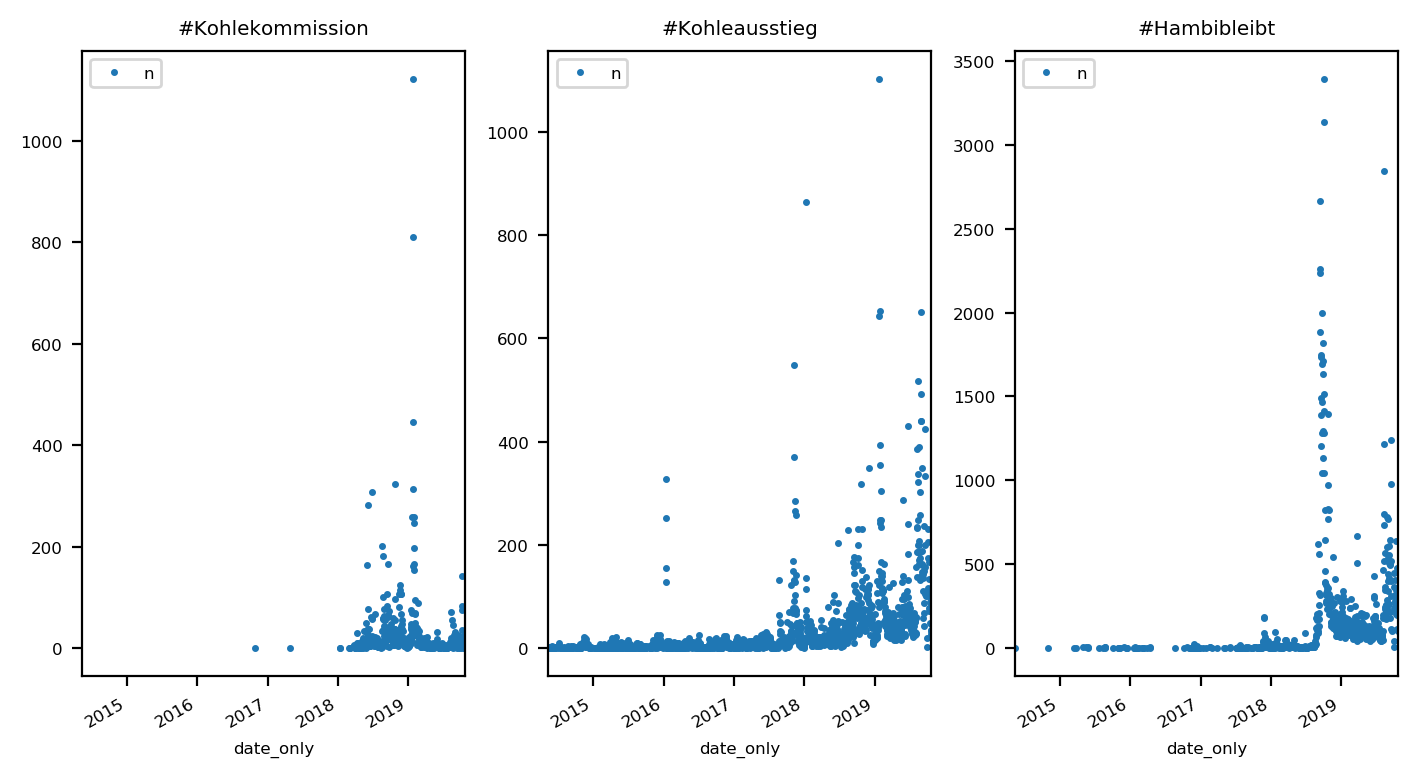
\includegraphics[width=0.8\linewidth]{figures/hashtags_time}
\end{center}
   \caption{Frequency of tweets containing relevant hashtags over time}
\label{fig:hashtags_time}
\end{figure}

\subsection{Method}
\paragraph{} In order to first detect significant events and topics of discussion, topic modelling will first be used. Topic modelling involves the use of a type of statistical model for discovering the abstract "topics" that occur in a collection of documents. Within this, an appropriate variant of topic modelling will be identified for best use, such as non-negative matrix factorisation (NMF) or latent Dirichlet allocation (LDA). It would be appropriate to use dynamic topic modelling here, in order to see the development of topics across time. This can be combined with looking at descriptive statistics like the frequency of tweets across time, in order to discern what social media users talk about and when. 

\begin{figure*} 
	\begin{center}
		\includegraphics[width=0.8\linewidth]{figures/gantt_chart}
	\end{center}
	\caption{Frequency of tweets containing relevant hashtags over time}
	\label{fig:gantt_chart}
\end{figure*}

\paragraph{} Next, in order to aggregate public opinion on Twitter, sentiment analysis can be used. Sentiment analysis refers to the use of natural language processing and text analysis to systematically identify and extract affective states and subjective information in text. In this project, besides analysing what social media users are talking about regarding the coal commission process, it is important to understand how they phrase their statements as well, in order to get an understanding of their opinion on a topic. 

\paragraph{} Finally, a measure to detect the polarisation of tweets would be important for analysis. This can be manifested by looking at text scaling methods and comparing tweets to a reference baseline. Another interesting method would be to utilise the unique structure of tweets, by looking at the retweet network of the tweets in order to determine whether there is a change in the network over time, thereby signifying some sort of change in positions. Further research would have to be conducted in this area in order to determine an appropriate measure for measuring polarisation. 

\subsection{Baseline}

\paragraph{} In this project, the baseline assumption is that there is no change in public opinion over the process of the coal commission, and that the multi-stakeholder expert commission process does not lead to any consensus building. The reference baseline, therefore, would be the public opinion at the beginning of the coal commission process, which can be measured by taking a time slice of tweets when the commission was first formed and measuring sentiment and polarisation at that time. 

\subsection{Evaluation}

\paragraph{} A successful outcome of this project would be an assessment on whether the coal commission process led to the building of a consensus amongst the public, following through the tasks and using the methods detailed in the previous sections. In particular, identifying and using a robust method to measure polarisation of tweets would be ideal.  

\section{Timeline}


\paragraph{} Figure \ref{fig:gantt_chart} shows a proposed Gantt chart for this project. The idea is to proceed simultaneously with background research and analysis, followed by writing and further analysis. 



{\small
\bibliographystyle{ieee}
\bibliography{bibliography.bib}
}

\end{document}
